% Source of the journal-format manuscript of article 3 (Izvestiya RAN, Ser. Geogr., rules of 17.11.2025).
% Citation placeholders and the two bibliography markers are expanded by
% tools/build_article3_journal.py into article3_v2.tex (plain-text author-year citations).
\documentclass[12pt,a4paper]{article}
\usepackage[a4paper,top=2cm,bottom=2cm,left=3cm,right=1.5cm]{geometry}
\usepackage{iftex}
\ifPDFTeX
  \usepackage[T2A]{fontenc}
  \usepackage[utf8]{inputenc}
  \usepackage[russian]{babel}
\else
  \usepackage{fontspec}
  \usepackage{polyglossia}
  \setdefaultlanguage{russian}
  \setotherlanguage{english}
  \defaultfontfeatures{Ligatures=TeX}
  \IfFontExistsTF{Times New Roman}{%
    \setmainfont{Times New Roman}\newfontfamily\cyrillicfont{Times New Roman}%
  }{%
    \IfFontExistsTF{Liberation Serif}{%
      \setmainfont{Liberation Serif}\newfontfamily\cyrillicfont{Liberation Serif}%
    }{\setmainfont{CMU Serif}\newfontfamily\cyrillicfont{CMU Serif}}%
  }
\fi
\usepackage{setspace}
\usepackage{mathtools,amssymb}
\usepackage{graphicx}
\usepackage{booktabs}
\usepackage{array}
\usepackage{caption}
\captionsetup{labelsep=period,font=normalsize,justification=raggedright,singlelinecheck=false}
\usepackage{titlesec}
\titleformat{\section}{\normalfont\bfseries\centering}{}{0pt}{}
\titleformat{\subsection}{\normalfont\itshape}{}{0pt}{}
\titlespacing*{\section}{0pt}{18pt}{6pt}
\titlespacing*{\subsection}{0pt}{12pt}{3pt}
\usepackage[unicode,hidelinks]{hyperref}
\setlength{\parindent}{1.25cm}
\setlength{\emergencystretch}{3em}
\hyphenpenalty=10000 \exhyphenpenalty=10000
\onehalfspacing
\pagestyle{plain}

\begin{document}

\noindent УДК 551.513

\begin{center}
{\large\bfseries Иерархия атмосферной циркуляции: закон наследования между масштабными уровнями и его значение для районирования}

\medskip
{\bfseries Н. С. Сотириади\textsuperscript{*}}

Независимый исследователь, Москва, Россия

\textsuperscript{*}E-mail: n.sotiriadi@gmail.com
\end{center}

\begin{singlespace}
\noindent\textbf{Аннотация.} Атмосферная циркуляция устроена как иерархия: внутри циклонов и антициклонов размером в тысячи километров живут вихри в сотни километров, а внутри них -- вихри в десятки километров. В двух предыдущих статьях серии показано, что согласованность размещения соседних уровней этой иерархии (сопряженность уровней) -- устойчивая характеристика территории, и построена ее планетарная карта. Цель настоящей работы -- установить, по какому правилу связаны между собой уровни иерархии, и дать карте сопряженности единое объяснение. По полю относительного вихря на поверхности 850 гПа (реанализ ERA5, 2023--2024 гг.) для двенадцати областей размером 2000 на 2800 км и для 902 ячеек планетарной сетки измерена согласованность размещения всех пар уровней от 50 до 1600 км сверх той, что задана спектром поля. Найден простой закон: согласованность двух уровней зависит только от более крупного из них и не зависит от того, насколько мелок второй. Иначе говоря, каждый крупный уровень передает один и тот же рисунок размещения всем уровням ниже себя. Закон выполняется во всех 902 ячейках, не зависит от размера области и от режима циркуляции и воспроизводится в модельном расчете без усвоения наблюдений, то есть не сводится к особенностям реанализа и указывает на свойство атмосферной динамики. Сопряженность соседних уровней оказывается нормированной силой этого наследования. В исследованном диапазоне размеров территории различаются не устройством иерархии, а силой наследования; ее карта и есть карта сопряженности. Закон дает планетарной карте единое основание и позволяет использовать ее в районировании как характеристику устройства циркуляции.

\smallskip
\noindent\textbf{Ключевые слова:} иерархия геосистем, масштабные уровни, межуровневые связи, каскад, инвариант, реанализ, модельный расчет, внетропические циклоны, глубокая конвекция, районирование.
\end{singlespace}

\section{ПОСТАНОВКА ПРОБЛЕМЫ}

Атмосферная циркуляция устроена как лестница размеров. На верхней ступени -- циклоны и антициклоны в тысячи километров. Внутри них -- вихри и полосы облаков в сотни километров. Внутри тех -- вихри в десятки километров, и так до отдельных облаков. Каждая ступень этой лестницы изучена по отдельности: известно, где и как часто возникают циклоны (Chang et al., 2002; Hoskins, Hodges, 2005; Hoskins, Valdes, 1990), где сосредоточена глубокая конвекция (Feng et al., 2021; Houze, 2004), как распределена энергия по размерам (Nastrom, Gage, 1985). Гораздо меньше известно о том, как ступени связаны друг с другом: повторяют ли мелкие вихри рисунок крупных или размещаются независимо от них.

Этот вопрос -- географический. Иерархичность признана основным свойством геосистем (Сочава, 1978; Bertrand, 1968), а связи между уровнями иерархии -- одной из главных задач ландшафтоведения (Пузаченко, 1986; Хорошев, 2016). Для ландшафта такие связи измерены: показано, какая часть свойств участка задана геосистемами более высокого ранга, а какая складывается на самом участке (Хорошев, 2016; Хорошев и др., 2010); найдены уровни организации регионального климата (Кренке и др., 2019); предложено рассматривать инварианты ландшафта как параметры порядка динамической системы (Байбар и др., 2023). В общей теории иерархических систем сформулировано понятие почти-разложимости: уровни связаны слабо, и потому каждый из них можно изучать отдельно (Simon, 1962; Simon, Ando, 1961); верхний уровень ограничивает нижний, а нижний дает механизм (O'Neill et al., 1986; Wu, 1999). Однако количественной меры силы связи между уровнями эта теория не дала, а для атмосферы связи между уровнями не измерялись и не картировались.

В первых двух статьях серии\footnote{Сотириади Н. С. Сопряженность иерархических уровней атмосферной циркуляции как региональный инвариант (первая статья серии; подана в печать); Сотириади Н. С. География сопряженности иерархических уровней атмосферной циркуляции: планетарная карта, ее факторы и районирование (вторая статья серии; подана в печать). Программы, протоколы проверок и результаты расчетов настоящей работы открыты: https://github.com/Theclimateguy/Shroedinger (дата обращения 22.09.2026); постоянный архив -- Zenodo, doi: 10.5281/zenodo.19565769.} такая мера предложена и проверена. Это сопряженность соседних масштабных уровней $P$ -- согласованность размещения изменчивости двух соседних уровней сверх той, что задана спектром поля; сопряженность есть характеристика одновременного размещения, а не переноса энергии или причинного воздействия между уровнями. Показано, что $P$ -- устойчивая характеристика территории: она не зависит от сезона, года, источника данных и способа разбиения территории и воспроизводится в модельном расчете без усвоения наблюдений (статья~I). Построена ее планетарная карта: наибольшие значения -- над путями внетропических циклонов, наименьшие -- над очагами глубокой конвекции; предложена схема районирования (статья~II).

Карта была получена, но не объяснена. Неизвестно, по какому правилу связаны уровни: касается ли связь только соседних ступеней или тянется через всю лестницу; одинаково ли устроена иерархия в разных частях планеты или различается; и чем является сама величина $P$ -- одной из многих возможных мер связи или естественной характеристикой устройства иерархии. Без ответа на эти вопросы карта остается описанием, а не характеристикой устройства циркуляции, и ее место в районировании остается неясным.

\emph{Цель работы} -- установить закон, по которому связаны масштабные уровни атмосферной циркуляции, и на его основе дать единое объяснение сопряженности уровней и ее планетарной карте. Задачи: (1) измерить согласованность размещения всех пар уровней, а не только соседних; (2) найти правило, которому подчиняются эти согласованности, и проверить его на независимых носителях -- на крупных областях, на планетарной сетке ячеек и в модельном расчете; (3) показать, как сопряженность соседних уровней $P$ следует из найденного правила; (4) сформулировать, что найденный закон дает районированию.

\section{ДАННЫЕ И МЕТОДИКА ИССЛЕДОВАНИЯ}

Данные, построение уровней и вычисление сопряженности полностью описаны в статьях~I--II; здесь они повторены в объеме, нужном для чтения результатов. Используется поле относительного вихря на поверхности 850 гПа реанализа ERA5 (Hersbach et al., 2020; Soci et al., 2024) с шагом 0.25$^\circ$ и 6 ч. Поле разложено на шесть масштабных уровней -- полос размеров: менее 50 км, 50--100, 100--200, 200--400, 400--800 и 800--1600 км (каждая следующая вдвое крупнее). Для каждого уровня строится карта его активности -- сглаженный модуль изменчивости данного размера, взятый в логарифме (далее -- огибающая уровня). Согласованность размещения двух уровней измеряется как корреляция их огибающих по территории в каждый срок; итог -- медиана по срокам.

Существенная часть согласованности любых двух уровней задана спектром поля -- распределением энергии по размерам -- и перекрытием соседних полос. Чтобы выделить только ту часть, которая отражает устройство иерархии, применяется суррогатная поправка (статья~I): строятся 99 полей с тем же спектром, но со случайными фазами (Basu et al., 2007), для них вычисляется та же согласованность, и ее медиана вычитается из наблюденной. Все величины ниже -- с этой поправкой; их называют сверхспектральными. Согласованность используется в двух формах: как корреляция (безразмерная, от $-1$ до 1; для соседних уровней это и есть $P$) и как ковариация логарифмов огибающих (в единицах дисперсии; далее -- $C$).

Расчеты выполнены на трех носителях. Первый -- двенадцать областей первой статьи размером 2000 на 2800 км, по четыре трехмесячных окна (зимы и лета 2023 и 2024 гг.), 48 единиц; здесь доступна полная лестница уровней до 1600 км. Второй -- 902 ячейки планетарной сетки второй статьи размером около 700 км между 60$^\circ$ ю.ш. и 60$^\circ$ с.ш. (два сезона 2023 г.; исключены ячейки со средней высотой рельефа более 1200 м); в ячейках такого размера лестница ограничена уровнем 400 км. Третий -- свободный расчет климатической модели ECMWF-IFS-HR (Haarsma et al., 2016; Roberts et al., 2018) без усвоения наблюдений (шаг 0.5$^\circ$, 2014 г.), в тех же двенадцати областях. Для проверки зависимости от размера области двенадцать областей пересчитаны при уменьшении сторон до 0.7 исходных (1400 на 1960 км).

Все проверки выполнены по протоколам, зафиксированным до расчетов: заранее записаны проверяемые утверждения, статистики, пороги и правила решения. Отклонения от протоколов и все разведочные расчеты, не входившие в протоколы, помечены в тексте явно. Статистическая значимость на двенадцати областях оценивается знаковым ранговым критерием (единица вывода -- область, среднее по ее окнам); на планетарной сетке -- блочным бутстрэпом по блокам 30 на 30$^\circ$ и нулевым распределением, полученным вращением карт по долготе (статья~II).

\section{РЕЗУЛЬТАТЫ ИССЛЕДОВАНИЯ}

\subsection{Связь тянется через всю лестницу уровней}

Первый вопрос -- касается ли согласованность только соседних уровней. Ответ отрицательный. На двенадцати областях сверхспектральная корреляция огибающих уровней, разделенных одной ступенью (например, 50 и 200 км), составляет в среднем по области 0.35 и положительна во всех двенадцати областях (от 0.29 до 0.48; $p = 0.0002$). Для соседних уровней та же величина равна 0.27. Далее по лестнице связь убывает: через две ступени 0.25, через три 0.16, через четыре (50 и 1600 км) 0.09, но остается значимой. На планетарной сетке связь через ступень составляет 0.36 с доверительным интервалом 0.35--0.37.

Важно, что для несоседних уровней суррогатная поправка почти не нужна: полосы не перекрываются, и согласованность у случайно-фазовых полей близка к нулю (0.16 через одну ступень, 0.02 через две, менее 0.01 через четыре), тогда как у наблюденных полей она равна 0.64, 0.41, 0.21 и 0.10. Иначе говоря, связь между далекими уровнями видна в исходных данных без всякой обработки. Для соседних уровней, напротив, наблюденная корреляция 0.87 на две трети состоит из перекрытия полос. Отсюда следует, что изменчивость мелкого уровня воспроизводит пространственный рисунок не только ближайшего крупного уровня, но и всех уровней выше него, вплоть до масштаба циклонов.

\subsection{Закон наследования: согласованность зависит только от более крупного уровня}

Второй вопрос -- по какому правилу убывает связь. Для его решения на двенадцати областях вычислена сверхспектральная ковариация $C$ огибающих всех пятнадцати пар уровней (рис.~2). В матрице видна простая закономерность: числа в каждом столбце почти одинаковы, а между столбцами различаются в разы. Столбец -- это более крупный уровень пары. Ковариация уровня 400 км с уровнем 50 км равна 0.131, с уровнем 100 км -- 0.143, с уровнем 200 км -- 0.143. Ковариация уровня 1600 км с уровнями 50, 100, 200, 400 и 800 км равна 0.012, 0.012, 0.013, 0.016 и 0.019. Таким образом, согласованность двух уровней задана более крупным из них и почти не зависит от того, насколько мелок второй.

Это утверждение проверено формально. Для каждой единицы (область и окно) десять ковариаций несоседних пар описаны двумя способами: как функция более крупного уровня и как функция расстояния между уровнями (числа ступеней). Первое описание объясняет 99.6\,\% изменчивости ковариаций, второе -- 27\,\%; разность, усредненная по области, положительна во всех двенадцати областях (от 0.62 до 0.83 при пороге 0.10; $p < 10^{-4}$). На планетарной сетке, где доступны три несоседние пары, закон предсказывает, что ковариации пар (50, 400) и (100, 400) равны, а пар (50, 200) и (100, 400) -- нет. Разность первых составляет 5\,\% от разности вторых (доверительный интервал 4.8--5.7\,\%), и это соотношение выполняется в 100\,\% из 902 ячеек (рис.~4). Оно не связано ни с конвективной неустойчивостью, ни с активностью циклонов (ранговые корреляции $-0.005$ и $0.02$): в исследованном диапазоне размеров устройство иерархии одинаково в тропиках и в умеренных широтах, над сушей и над океаном.

В словесной форме закон таков. Каждый крупный уровень передает всем уровням ниже себя один и тот же рисунок размещения, а мелкий уровень получает свой рисунок от всех уровней выше себя; согласованность двух уровней -- это общая для них часть рисунка, унаследованная от их общего крупного уровня. Здесь и далее “наследование” обозначает статистическое воспроизведение пространственного рисунка одного уровня на другом, а не установленный физический процесс переноса энергии или причинного воздействия: измеряется одновременное размещение уровней, и направления передачи оно не задает. В формульной записи: если $E(a)$ -- огибающая уровня размера $a$, а $G(a)$ -- изменчивость рисунка, унаследованного от уровня $a$ и всех уровней крупнее, то
\begin{equation}
C\bigl(E(a),\,E(a')\bigr) = G\bigl(\max(a,\,a')\bigr).
\label{eq:law}
\end{equation}
Величина $G(a)$ убывает с ростом $a$ (рис.~3): от 0.25 при 200 км до 0.12 при 400, 0.04 при 800 и 0.01 при 1600 км, примерно как степенная функция размера с показателем около $-1.5$. Такая зависимость известна в теории каскадов турбулентности как признак передачи изменчивости от крупных вихрей к мелким через цепочку промежуточных (Arneodo et al., 1998; Lovejoy, Schertzer, 2013); для атмосферной циркуляции она установлена впервые.

\subsection{Закон не зависит от размера области и от инструмента}

Найденное правило могло быть свойством способа измерения или реанализа, а не атмосферы. Три проверки говорят против этого. Во-первых, при уменьшении сторон областей до 0.7 исходных форма зависимости $G(a)$ не меняется: отношение значений, полученных на малых и на исходных областях, составляет 0.93--1.02 по всем двенадцати областям; меняется лишь общий уровень ковариаций (в среднем на 20\,\% ниже). Во-вторых, закон выполняется в свободном расчете климатической модели, которая не использует наблюдений: разность двух описаний составляет 0.62--0.78 во всех двенадцати областях ($p < 10^{-4}$), а амплитуда $G(200~\text{км})$ по областям воспроизводится с ранговой корреляцией 0.93 (рис.~3б, табл.~1). В-третьих, закон одинаково выполняется на ячейках планетарной сетки и на крупных областях, хотя размер ячейки в три раза меньше.

\subsection{Сопряженность соседних уровней как сила наследования}

Третий вопрос -- чем является величина $P$ первых двух статей по отношению к найденному закону. Закон~(\ref{eq:law}) получен на несоседних парах, у которых нет перекрытия полос. Распространяется ли он на соседние пары, где перекрытие велико и снято только суррогатной поправкой? Проверка дает утвердительный ответ: ковариация соседних уровней после поправки равна величине $G$, оцененной по несоседним парам, с корреляцией 0.99 и средним отношением 1.02 на планетарной сетке, 1.06 на областях и 1.09 в модельном расчете. Таким образом, суррогатная поправка делает ровно то, для чего вводилась: снимает перекрытие полос и оставляет закон.

Отсюда следует смысл $P$. Корреляция -- это ковариация, деленная на разброс каждого из двух уровней. Значит, сопряженность соседних уровней $a$ и $a'$ есть
\begin{equation}
P \approx \frac{G(a')}{\sqrt{V(a)\,V(a')}},
\label{eq:P}
\end{equation}
где $V$ -- полная изменчивость огибающей уровня: унаследованный рисунок, отнесенный к общей изменчивости обоих уровней, -- нормированная сила наследования. На планетарной сетке правая часть~(\ref{eq:P}) связана с наблюденной $P$ ранговой корреляцией 0.63--0.64 по двум парам соседних уровней ($p = 0.001$; рис.~5), а по двенадцати областям -- 0.80. Наблюденная $P$ примерно вдвое меньше правой части: суррогатная поправка вычитает корреляцию случайно-фазовых полей, у которых разброс огибающих меньше, чем у наблюденных, и потому вычитает несколько больше нужного. Это сжатие одинаково по всем территориям и на ранжирование не влияет. По надежности карты $P$ и нормированная сила наследования равноценны (расщепленная надежность 0.72 и 0.71), а ненормированная амплитуда $G(200~\text{км})$ уступает им (0.79 против 0.87 у $P$ на полной сетке). Поэтому оценкой инварианта остается $P$.

Амплитуда наследования несет географию карты. По двенадцати областям ранговая корреляция $P$ с $G(200~\text{км})$ равна 0.82, на планетарной сетке -- 0.68. Амплитуда тесно связана с перемежаемостью огибающих -- разбросом логарифма активности, который в статье~II входил в число факторов карты (корреляция 0.93). При этом одно число $G(200~\text{км})$ описывает карту не хуже четырех статистик перемежаемости вместе: прибавка к качеству предсказания карты сверх восьми факторов статьи~II и блока перемежаемости составляет $+0.047$ ($p = 0.001$), а обратная прибавка блока сверх факторов и $G$ -- $+0.014$.

\section{ОБСУЖДЕНИЕ РЕЗУЛЬТАТОВ}

\subsection{Единое объяснение карты}

Найденный закон соединяет три статьи серии в одно рассуждение. На исследованных носителях и в диапазоне размеров от 50 до 1600 км устройство иерархии одно и то же, а территории различаются силой наследования -- тем, насколько велика унаследованная часть рисунка по сравнению с общей изменчивостью; карта сопряженности (статья~II) -- карта этой силы. Пути внетропических циклонов -- территории, где наследование сильно; очаги глубокой конвекции -- где оно слабо; конвекция и активность циклонов, найденные в статье~II как факторы карты, суть факторы амплитуды закона, а не его формы. Перемежаемость огибающих, входившая в статье~II в число факторов, оказывается проявлением того же наследования.

Закон описывает устройство иерархии, но не отвечает на вопрос, почему сила наследования распределена по планете именно так. Известно лишь, с чем она связана статистически: с активностью внетропических циклонов и с глубокой конвекцией (статья~II). Проверка двух правдоподобных объяснений -- растяжения воздуха внутри циклонов, которое должно было бы привязывать мелкомасштабную изменчивость к крупной (Hoskins, Bretherton, 1972), и глубокой конвекции, которая должна была бы размещать ее независимо от крупной (Craig, Cohen, 2006), -- показала, что растяжение воздуха есть везде и одинаково, а различий между территориями не несет. Механизм распределения амплитуды по карте остается предметом будущих исследований. Установленное здесь -- что закон выполняется без исключений на всех носителях, включая модельный расчет без усвоения наблюдений, и не зависит от режима циркуляции, -- указывает на свойство атмосферной динамики, не сводимое к особенностям реанализа или способа измерения.

\subsection{Место результата в науке о масштабной организации}

Форма измеряемой величины не нова. Корреляция логарифмов огибающих разных масштабов в пространстве и по размерам введена для рядов турбулентности (Arneodo et al., 1998) и применена к спутниковым изображениям облачности (Roux et al., 2000), к приземному слою атмосферы с той же суррогатной поправкой (Basu et al., 2007), к статистикам изображений и к полям крупномасштабной структуры Вселенной (Allys et al., 2020; Cheng et al., 2024); ее ближайший родственник в океанологии -- статистики рассеяния, которыми недавно различены два района Северной Атлантики с одинаковым спектром (Skinner et al., 2025). В метеорологии карты локальных спектров показали, что мезомасштабная изменчивость организована внутри огибающих крупного масштаба, с исключениями над очагами конвекции и горами (Kouhen et al., 2024; Wang, Sardeshmukh, 2021). Новое в настоящей работе -- не статистика, а объект: закон~(\ref{eq:law}) установлен для динамического поля атмосферы на планете в целом и связан с ранее введенной сопряженностью уровней. Тем самым сопряженность получает место в теории иерархических систем: это первая измеренная для атмосферы характеристика связи между уровнями -- того, что в ландшафтоведении называют межуровневыми связями (Хорошев, 2016) и оценивают как долю свойств участка, заданную геосистемами высшего ранга (Хорошев и др., 2010), а в общей теории иерархий -- как степень почти-разложимости (Simon, 1962).

\subsection{Значение для районирования}

Для районирования закон дает три вещи. Во-первых, основание: карта сопряженности делит территории по характеристике устройства циркуляции, а не по среднему состоянию, как схемы климатического районирования (Исаченко, 1991), и это устройство подчиняется простому закону. Во-вторых, экономию: территория описывается одним числом -- силой наследования; несколько статистик перемежаемости, которые пришлось бы вводить иначе, заменяются одной. В-третьих, единицу сравнения: две территории с одинаковой силой наследования устроены одинаково на всех исследованных уровнях, что дает основание выбирать территории-аналоги для региональных исследований мезомасштабных процессов. Схема районирования статьи~II при этом не меняется.

\subsection{Ограничения}

Уровни 50--200 км лежат ниже эффективного разрешения реанализа (Skamarock, 2004); закон на этих уровнях описывает поле реанализа, а не наблюдений, и подтвержден модельным расчетом с еще более грубым шагом. Абсолютные значения ковариаций зависят от размера области (на 20\,\% при уменьшении сторон на 30\,\%; в ячейках 700 км они в три--пять раз меньше, чем в областях 2000 км), поэтому сравнивать между работами можно только ранжирование территорий, а не значения. Закон проверен на пяти ступенях лестницы и на одном уровне давления; его выполнение на более крупных уровнях и на других уровнях давления не проверялось. Показатель убывания $G(a)$ (около $-1.5$) неустойчив по окнам и как характеристика территории не сообщается. Наконец, проверки статьи опираются на те же поля, из которых вычислена сопряженность; независимая проверка по другим переменным -- например, по полям осадков -- остается задачей будущего.

\section{ЗАКЛЮЧЕНИЕ}

1. Согласованность размещения масштабных уровней атмосферной циркуляции не ограничена соседними уровнями: изменчивость мелкого уровня воспроизводит пространственный рисунок всех уровней выше него, вплоть до масштаба циклонов; для несоседних уровней связь видна в исходных данных без суррогатной поправки.

2. Установлен закон: сверхспектральная согласованность двух уровней зависит только от более крупного из них и не зависит от расстояния между уровнями. Каждый крупный уровень передает всем уровням ниже один и тот же рисунок размещения. Закон объясняет 99.6\,\% изменчивости согласованностей на двенадцати областях, выполняется в 100\,\% из 902 ячеек планетарной сетки, не зависит от размера области и режима циркуляции и воспроизводится в модельном расчете без усвоения наблюдений, то есть указывает на свойство атмосферной динамики.

3. Сопряженность соседних уровней $P$ первых двух статей есть нормированная сила наследования -- амплитуда закона, отнесенная к общей изменчивости уровней; в исследованном диапазоне территории различаются этой силой, а не устройством иерархии.

4. Для районирования закон дает основание, экономию описания и единицу сравнения территорий; схема районирования второй статьи не меняется, а получает объяснение.

\section{ФИНАНСИРОВАНИЕ}

Работа выполнена без внешнего финансирования.

%%GOST_LIST%%

%%REFERENCES_LIST%%

\clearpage
\begin{singlespace}
\noindent Таблица 1. Амплитуда наследования $G(200~\text{км})$ и сопряженность соседних уровней $P$ по двенадцати областям: реанализ ERA5 (2023--2024 гг., четыре окна) и свободный расчет модели IFS-HR (2014 г., два окна)

\medskip
\noindent\begin{tabular}{@{}lccc@{}}
\toprule
Область & $G$, ERA5 & $G$, модель & $P$, ERA5\\
\midrule
Север Тихого океана & 0.366 & 0.267 & 0.30\\
Северная Атлантика & 0.348 & 0.239 & 0.31\\
Бассейн Конго & 0.345 & 0.209 & 0.29\\
Южная Атлантика & 0.317 & 0.217 & 0.29\\
Теплый бассейн Тихого океана & 0.292 & 0.159 & 0.33\\
Центральная Азия & 0.277 & 0.198 & 0.30\\
Австралия & 0.243 & 0.177 & 0.27\\
Южно-Тихоокеанская зона конвергенции & 0.242 & 0.173 & 0.28\\
Юг Южной Америки & 0.220 & 0.150 & 0.26\\
Индонезия & 0.196 & 0.087 & 0.25\\
Европа & 0.186 & 0.126 & 0.24\\
Амазония & 0.145 & 0.096 & 0.23\\
\midrule
Ранговая корреляция с $G$, ERA5 & -- & 0.93 & 0.82\\
\bottomrule
\end{tabular}
\end{singlespace}

\clearpage
\noindent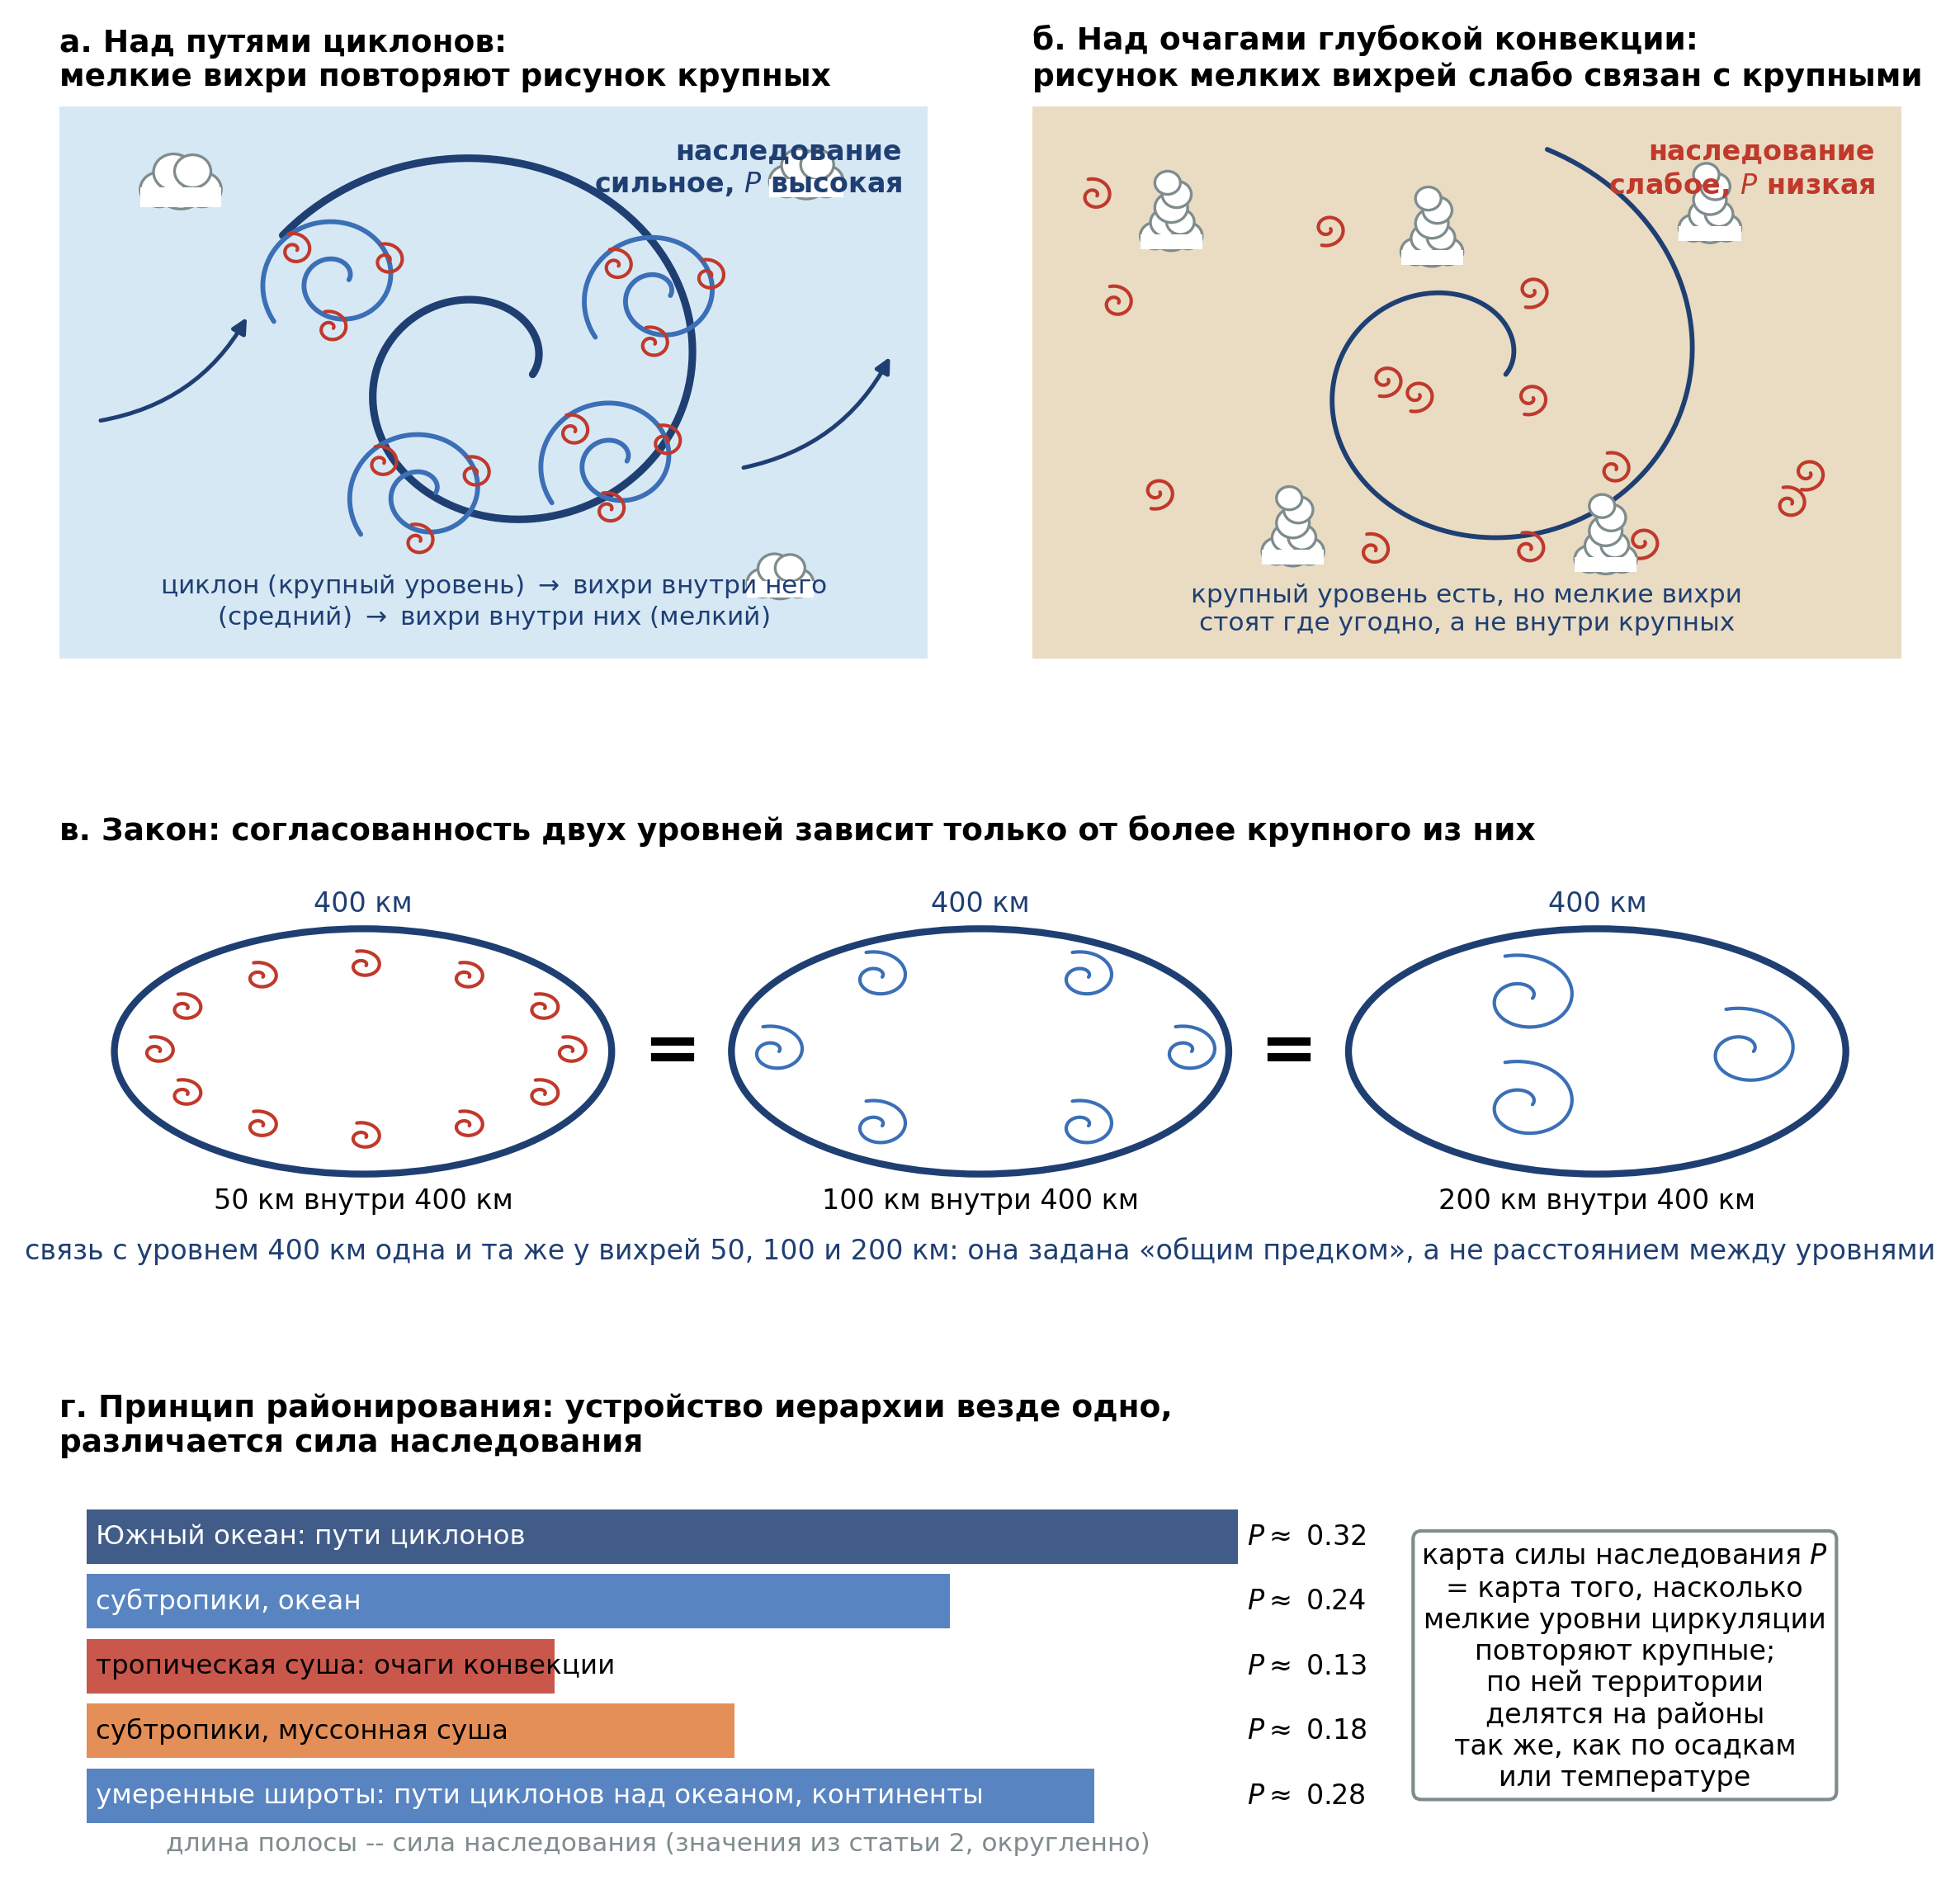
\includegraphics[width=\linewidth]{figures/ru_fig1_scheme_draw.png}

\noindent Рис. 1. Закон наследования между уровнями атмосферной циркуляции и принцип районирования (схема): а -- над путями циклонов мелкие вихри повторяют рисунок крупных, наследование сильное; б -- над очагами глубокой конвекции рисунок мелких вихрей слабо связан с крупными, наследование слабое; в -- согласованность двух уровней зависит только от более крупного из них; г -- устройство иерархии везде одно, территории различаются силой наследования, по которой и проводится районирование (значения $P$ по статье~II, округленно).

\clearpage
\noindent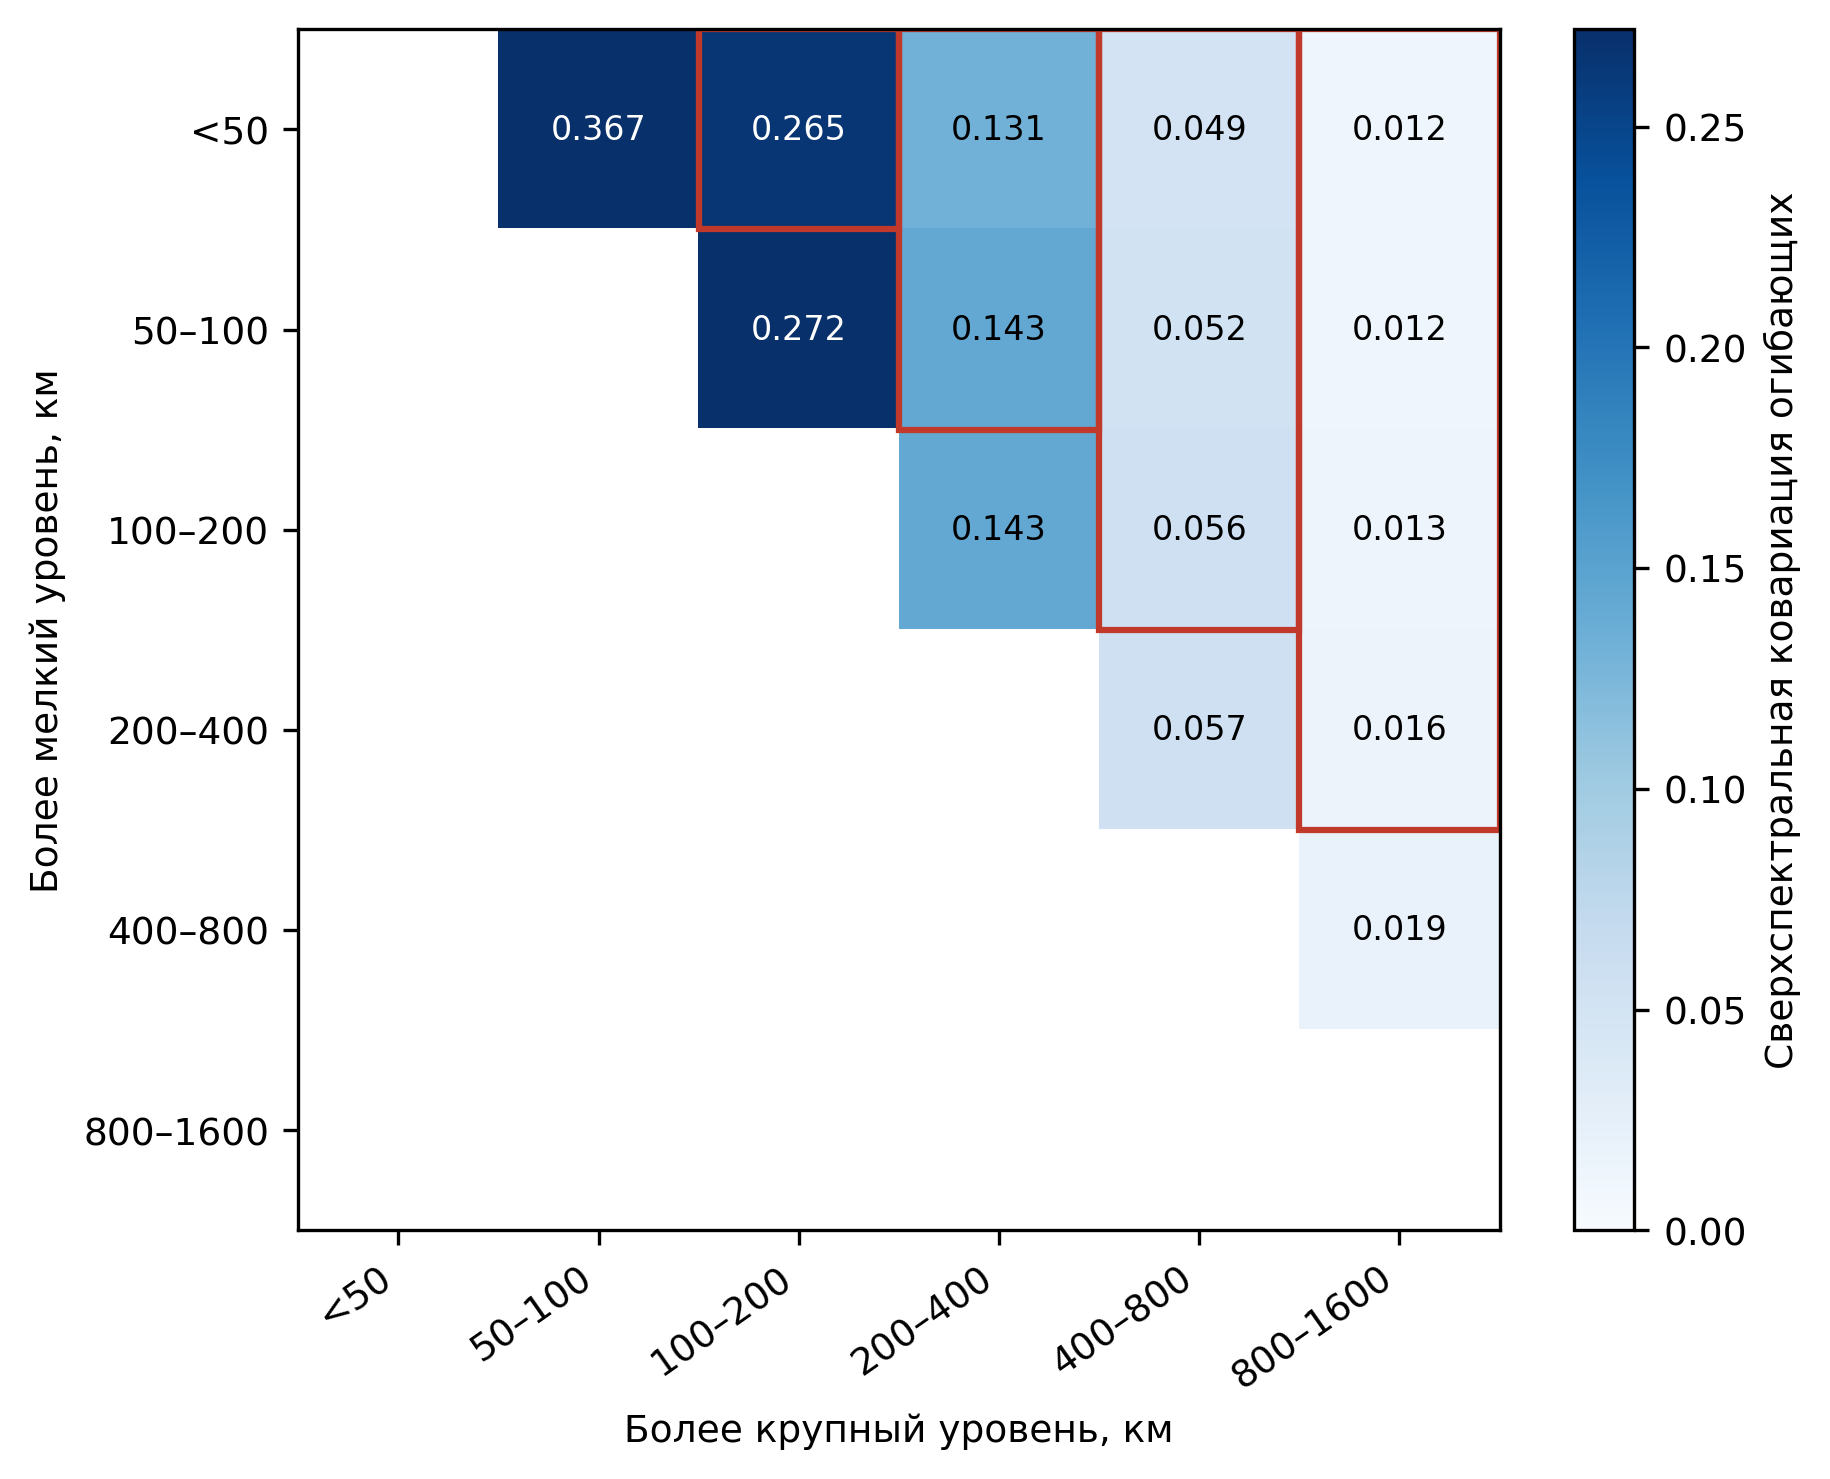
\includegraphics[width=0.85\linewidth]{figures/ru_fig2_matrix.png}

\noindent Рис. 2. Сверхспектральная ковариация огибающих всех пар масштабных уровней: среднее по двенадцати областям и четырем окнам (реанализ ERA5). Красными рамками выделены столбцы -- пары с одинаковым более крупным уровнем; значения внутри столбца почти одинаковы.

\clearpage
\noindent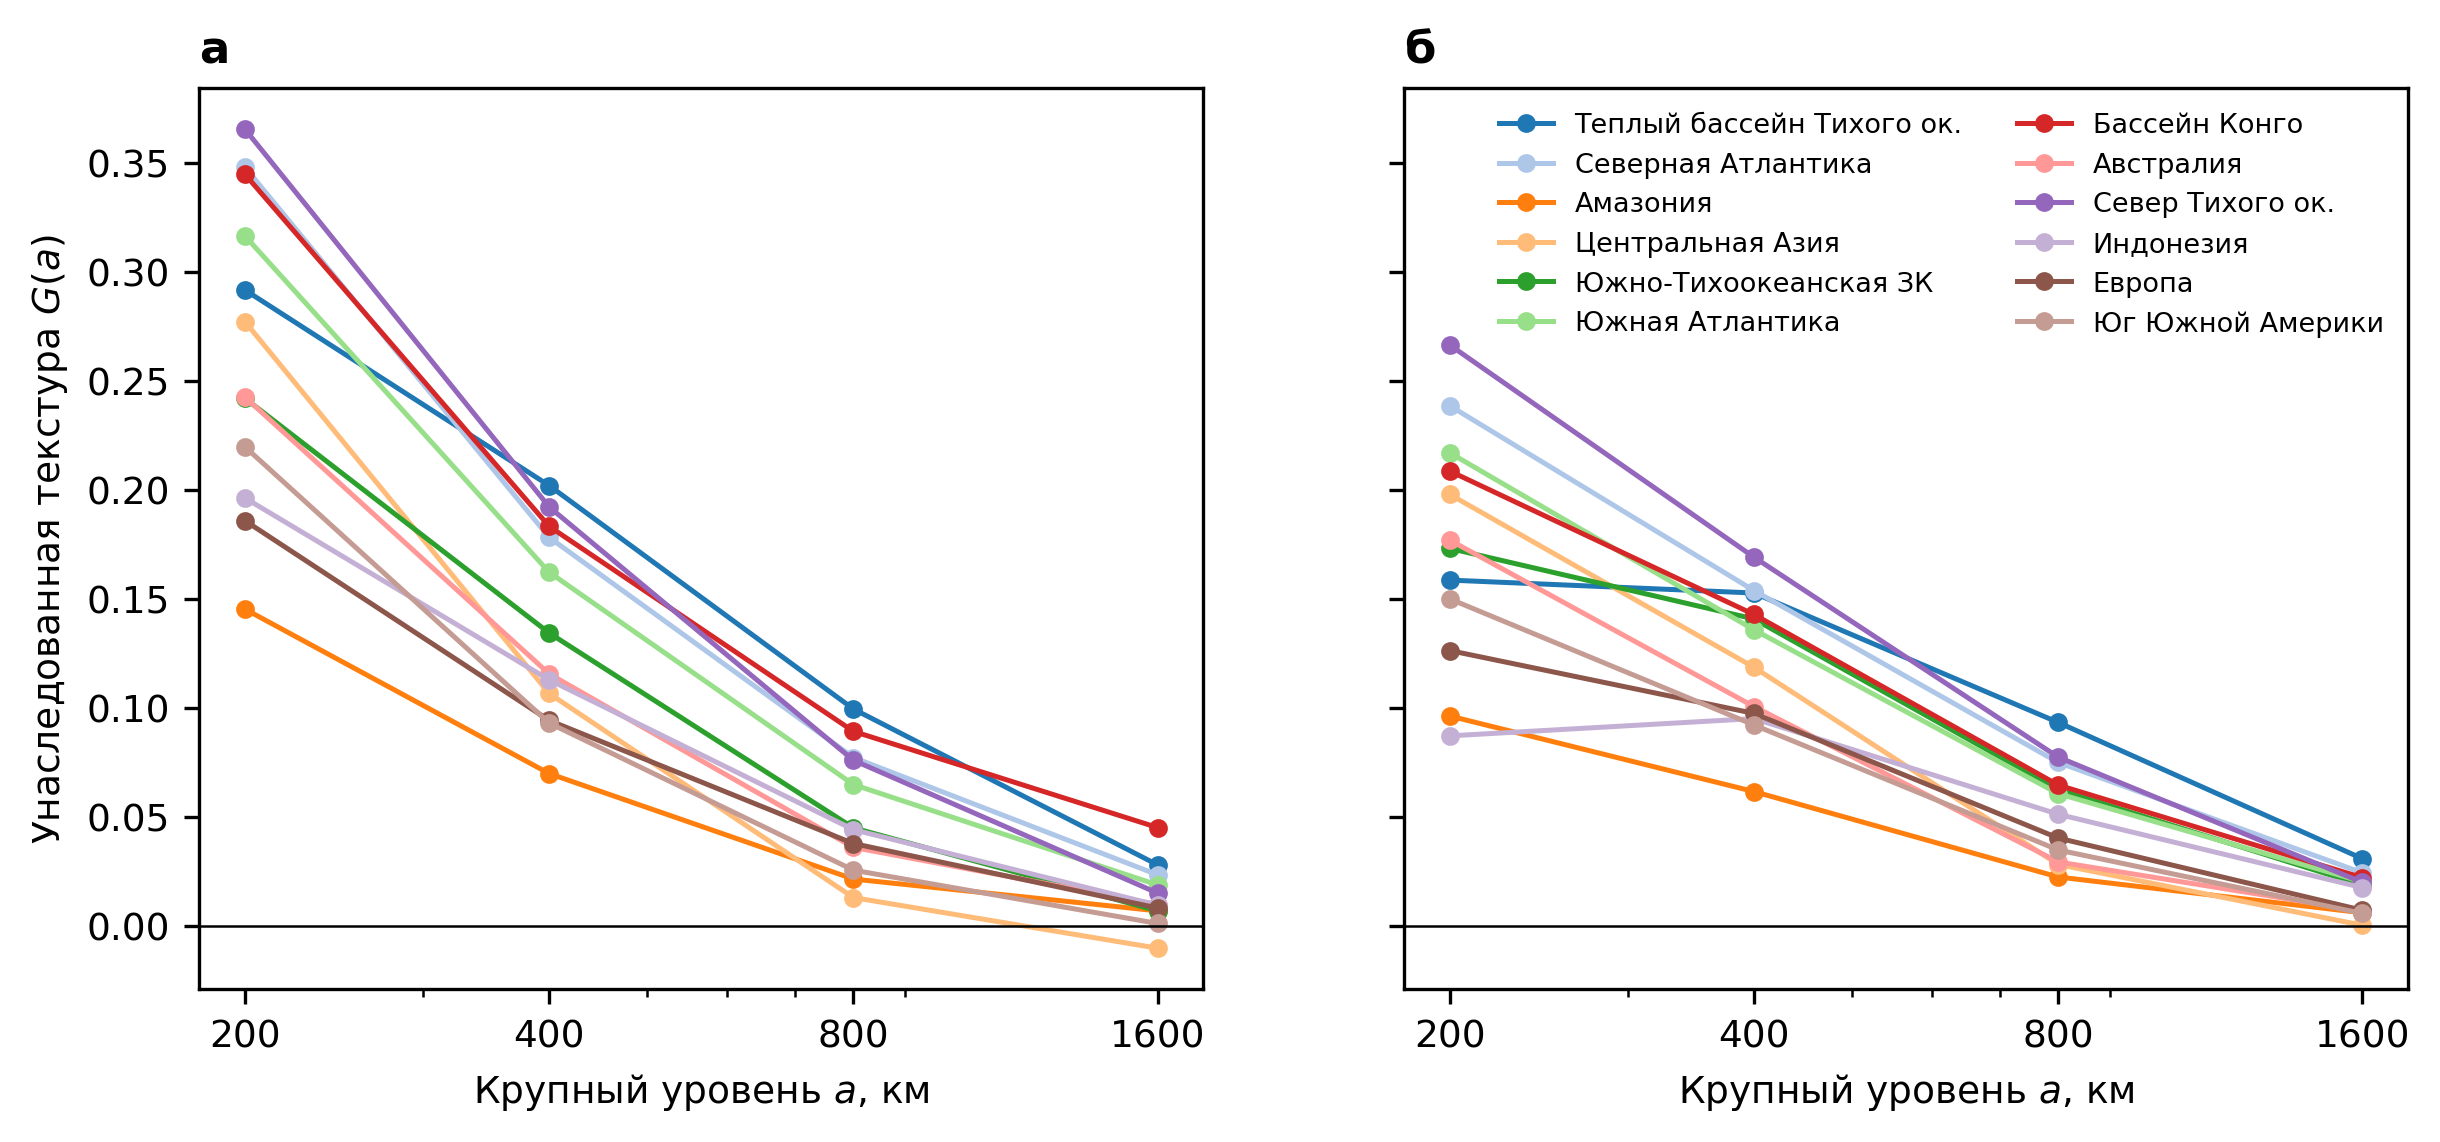
\includegraphics[width=\linewidth]{figures/ru_fig3_decay.png}

\noindent Рис. 3. Унаследованная изменчивость $G(a)$ в зависимости от размера крупного уровня $a$ по двенадцати областям: а -- реанализ ERA5, среднее по четырем окнам 2023--2024 гг.; б -- свободный расчет модели IFS-HR, среднее по двум окнам 2014 г.

\clearpage
\noindent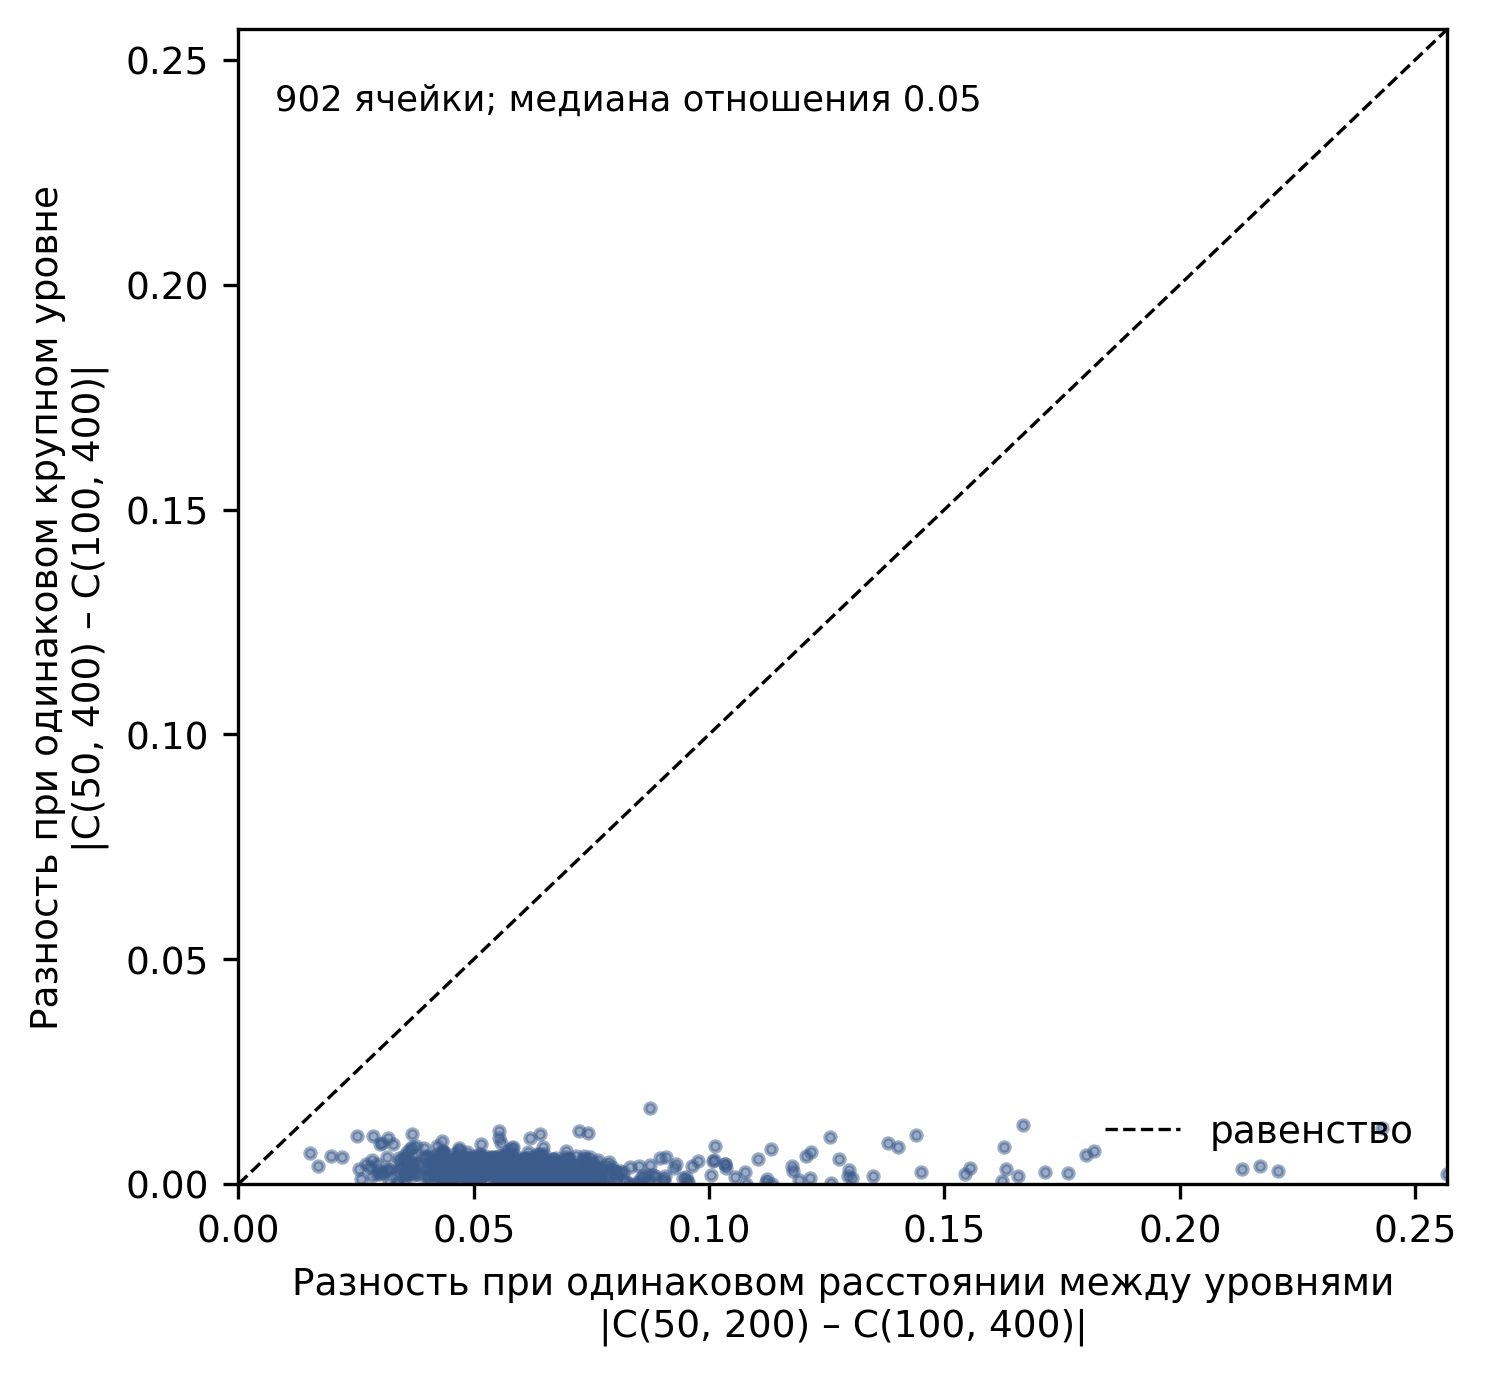
\includegraphics[width=0.7\linewidth]{figures/ru_fig4_tiles.png}

\noindent Рис. 4. Проверка закона на планетарной сетке (902 ячейки): разность ковариаций двух пар с одинаковым крупным уровнем (по вертикали) против разности двух пар с одинаковым расстоянием между уровнями (по горизонтали). Все точки лежат ниже линии равенства.

\clearpage
\noindent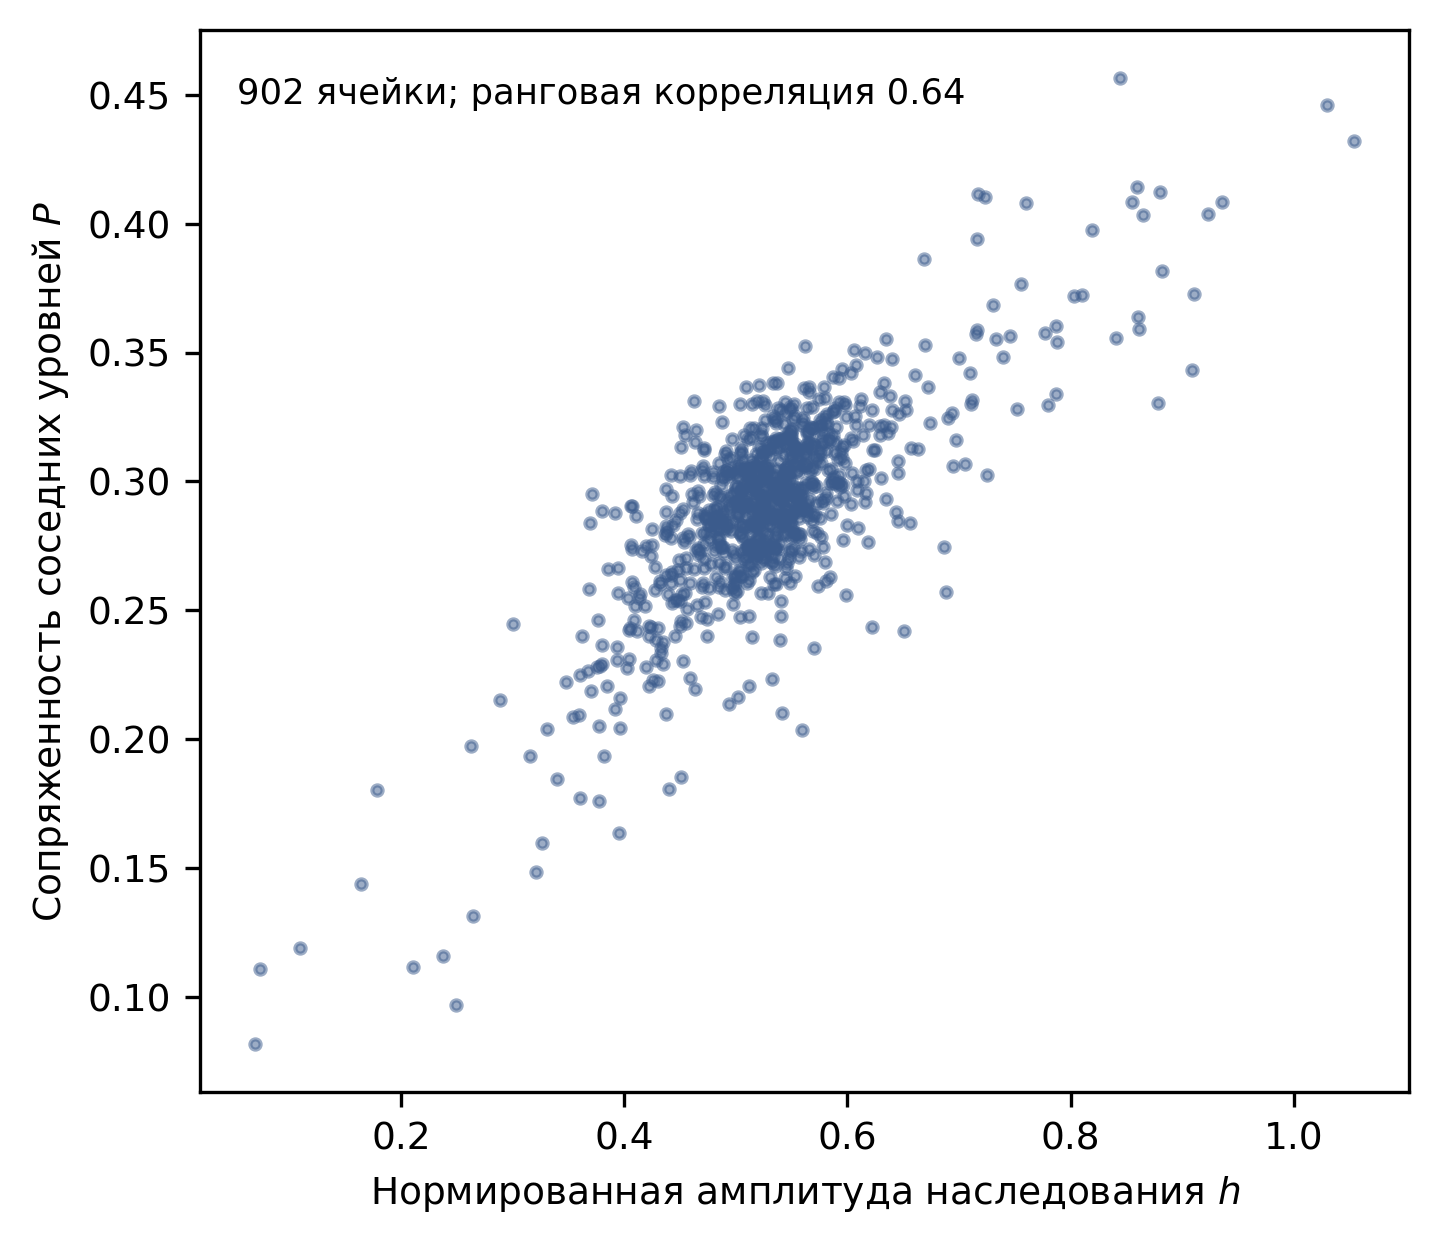
\includegraphics[width=0.7\linewidth]{figures/ru_fig5_P_vs_h.png}

\noindent Рис. 5. Сопряженность соседних уровней $P$ и нормированная сила наследования по формуле (2) на планетарной сетке (902 ячейки, среднее по парам уровней 100/200 и 200/400 км и по двум сезонам 2023 г.).

\clearpage
\begin{singlespace}
\noindent\textbf{Hierarchy of the atmospheric circulation: the law of inheritance between scale levels and its meaning for regionalisation}

\medskip
\noindent\textbf{N. S. Sotiriadi\textsuperscript{*}}

\noindent Independent researcher, Moscow, Russia

\noindent\textsuperscript{*}E-mail: n.sotiriadi@gmail.com

\medskip
\noindent\textbf{Abstract.} The atmospheric circulation is organised as a hierarchy: eddies of hundreds of kilometres live inside cyclones and anticyclones of thousands of kilometres, and eddies of tens of kilometres live inside them. The two previous papers of the series showed that the consistency of placement of adjacent levels of this hierarchy (inter-level coupling) is a stable property of territory and mapped it globally. The aim of this paper is to establish the rule by which the levels are related and to give the map a single explanation. Using the 850-hPa relative vorticity of the ERA5 reanalysis (2023--2024), the beyond-spectrum consistency of placement was measured for all pairs of levels from 50 to 1600 km in twelve 2000 by 2800 km regions and in 902 cells of a global grid. A simple law was found: the consistency of two levels depends only on the coarser of them and not on how fine the second is; each coarse level passes the same placement pattern to every level below it. The law holds in all 902 cells, is independent of the region size and of the circulation regime, and is reproduced by a climate-model run without data assimilation, hence it is not an artefact of the reanalysis and points to a property of the atmospheric dynamics. The coupling of adjacent levels is the normalised strength of this inheritance. Within the range of scales studied, territories differ not in the structure of the hierarchy but in the strength of inheritance; its map is the coupling map. The law gives the global map a single basis and allows it to be used in regionalisation as a property of the circulation structure.

\medskip
\noindent\textbf{Keywords:} hierarchy of geosystems, scale levels, inter-level links, cascade, invariant, reanalysis, model run, extratropical cyclones, deep convection, regionalisation.
\end{singlespace}

\end{document}
